\section{Stakeholders}

A continuación se detallan todos los interesados en el desarrollo del proyecto. Para generar la lista de los interesados se analizaron todos los posibles stakeholders que entraran en las siguientes categorías:
\begin{enumerate}
    \item Gerentes que definen los problemas del negocio que a menudo tienen una influencia significativa en el proyecto.
    \item Gerentes de proyectos (técnicos) que deben planificar, motivar, organizar y controlar a los profesionales que realizan el trabajo de software.
    \item Profesionales que brindan las habilidades técnicas necesarias par diseñar un producto o aplicación
    \item Clientes que especifican los requisitos para la ingeniería del software y otras partes interesadas que tienen un interés secundario en el resultado.
    \item Usuarios finales
\end{enumerate}
A esta clasificación se le suma el equipo anterior de desarrollo que cumplió la tarea de generar las primeras versiones del software que se va a mantener.
Luego para realizar la estimación de la influencia se refirió a la clasificación anterior, se analizó cuanto puede influir el stakeholder en el avance del proyecto, por lo que se generó la siguiente clasificación:

\begin{itemize}
    \item Alto: Tiene alto conocimiento en el dominio, o sus decisiones/acciones son cruciales para el avance del proyecto y la manera en la que avance
    \item Medio: Tiene un conocimiento básico del dominio o tiene una capacidad limitada o variable de generar incidencia en el proyecto.
    \item Bajo: Carece de la habilidad de generar requerimientos nuevos, su incidencia en el avnace del proyecto es minima.
\end{itemize}

Como último se analizó el interés en el desarrollo del proceso de software en sí, como del resultado después de la finalización del mismo, cada stackholder se evaluó con interés entre bajo y alto. Además de la clasificación sobre si es interno al equipo de desarrollo.

\prettyTable{|l|l|l|l|l|l|l|}
{
    \textbf{Nombre} & \textbf{Empresa} & \textbf{Rol} & \textbf{Influencia} & \textbf{Interés} & \textbf{Clasificación} \\ \hline
    Marcelo Plada & n/a & Equipo de desarrollo & Alto & Alto & Interno \\ \hline
    Vincent Silva & n/a & Equipo de desarrollo & Alto & Alto & Interno \\ \hline
    n/a & Animales sin hogar & Dirección & Alto & Alto & Externo \\ \hline
    n/a & Animales sin hogar & Usuario final & Bajo & Bajo & Externo \\ \hline
    n/a & n/a & Equipo anterior de desarrollo & Bajo & Bajo & Externo \\ \hline
    n/a & n/a & Cuerpo docente & Bajo & Alto & Externo \\ \hline
}

A continuación se va a realizar un análisis de importancia de los interesados encontrados en una matriz en función de el interés que tienen de avance del proyecto versus la influencia que tienen en el avance del proyecto. Para luego decidir el nivel de comunicación que se necesita por cada interesado.

\begin{figure}[H]
    \centering
    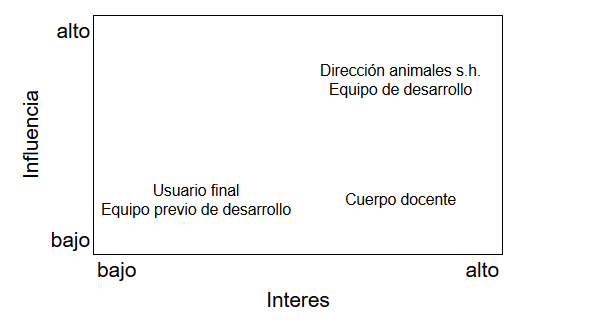
\includegraphics[scale=0.6]{Files/stakeholdersMatrix.png}
    \caption{Matriz de análisis para los interesados}
    \label{fig:clases}
\end{figure}

De el análisis se observa que los interesados más importantes son la dirección de animales sin hogar y el equipo de desarrollo. De esto se desprende que se deberá mantener un régimen de comunicación frecuente con los miembros de la dirección de animales sin hogar, donde se les notificará el estado del proyecto lo más frecuente posible y se les invitará a participar activamente en la propuesta de nuevas funcionalidades. El equipo de desarrollo encargado de realizar la aplicación también debe mantener una comunicación fluida ya que es una necesidad crítica la de mantener a todo el equipo comunicado.
El cuerpo de profesores que planteó el proyecto tienen una influencia alta al principio pero mas adelante no es tan fuerte, no así su interés el cual es alto durante todo el transcurso del proyecto por lo que se mantendrá informado de los cambios realizando las entregas periódicas pero no tendrán un efecto sobre las funcionalidades a realizar.

\begin{comment}

1. Gerentes sénior que definen los problemas comerciales que a menudo tienen una influencia significativa en el proyecto.
2. Gerentes de proyectos (técnicos) que deben planificar, motivar, organizar y controlar a los profesionales que realizan el trabajo de software.
3. Profesionales que brindan las habilidades técnicas necesarias para diseñar un producto o aplicación.
4. Clientes que especifican los requisitos para la ingeniería del software y otras partes interesadas que tienen un interés periférico en el resultado.
5. Usuarios finales

31.2.1 The Stakeholders
The software process (and every software project) is populated by stakeholders
who can be categorized into one of fi ve constituencies:
1. Senior managers who defi ne the business issues that often have a signifi -
cant infl uence on the project.
2. Project (technical) managers who must plan, motivate, organize, and control
the practitioners who do software work.
3. Practitioners who deliver the technical skills that are necessary to engineer
a product or application.
4. Customers who specify the requirements for the software to be engineered
and other stakeholders who have a peripheral interest in the
outcome.
5. End users

Se identifican los interesados internos y
externos al equipo. Se describe el tipo de
interés, particularmente si es positivo o
negativo. Se realiza un análisis de los objetivos
e influencia de los interesados en el proyecto.


nombre: nombre del interesado
posicion: la posicion que tiene el interesado en la empresa
rol: el rol que tiene el interesado en el equipo de desarrollo
contact information: informacion de contacto del stakeholder, email, telefono, direccion de la cassa
requerimientos: requerimientos de alto nivel para el proyecto y/o el producto
expectativas: principales expectativas para el proyecto y/o el producto
influencia: el grado de influencia que el interesado tiene sobre el proyecto, este puede ser descripto o mediante la utilizacion de una palabra clave
clasificacion: se podria clasificar como amigo, enemigo o neutral. u otra clasificacion como alto medio o bajo impacto


Identification information. Name, organizational position, location and
contact details, and role on the project.
Assessment information. Major requirements, expectations, potential for
influencing project outcomes, and the phase of the project life cycle where the
stakeholder has the most influence or impact.
Stakeholder classification. Internal/external, impact/influence/power/interest,
upward/downward/outward/sideward, or any other classification model chosen
by the project manager.


\end{comment}